% Options for packages loaded elsewhere
\PassOptionsToPackage{unicode}{hyperref}
\PassOptionsToPackage{hyphens}{url}
%
\documentclass[
  ignorenonframetext,
  aspectratio=169,
]{beamer}
\usepackage{pgfpages}
\setbeamertemplate{caption}[numbered]
\setbeamertemplate{caption label separator}{: }
\setbeamercolor{caption name}{fg=normal text.fg}
\beamertemplatenavigationsymbolsempty
% Prevent slide breaks in the middle of a paragraph
\widowpenalties 1 10000
\raggedbottom
\setbeamertemplate{part page}{
  \centering
  \begin{beamercolorbox}[sep=16pt,center]{part title}
    \usebeamerfont{part title}\insertpart\par
  \end{beamercolorbox}
}
\setbeamertemplate{section page}{
  \centering
  \begin{beamercolorbox}[sep=12pt,center]{part title}
    \usebeamerfont{section title}\insertsection\par
  \end{beamercolorbox}
}
\setbeamertemplate{subsection page}{
  \centering
  \begin{beamercolorbox}[sep=8pt,center]{part title}
    \usebeamerfont{subsection title}\insertsubsection\par
  \end{beamercolorbox}
}
\AtBeginPart{
  \frame{\partpage}
}
\AtBeginSection{
  \ifbibliography
  \else
    \frame{\sectionpage}
  \fi
}
\AtBeginSubsection{
  \frame{\subsectionpage}
}

\usepackage{amsmath,amssymb}
\usepackage{iftex}
\ifPDFTeX
  \usepackage[T1]{fontenc}
  \usepackage[utf8]{inputenc}
  \usepackage{textcomp} % provide euro and other symbols
\else % if luatex or xetex
  \usepackage{unicode-math}
  \defaultfontfeatures{Scale=MatchLowercase}
  \defaultfontfeatures[\rmfamily]{Ligatures=TeX,Scale=1}
\fi
\usepackage{lmodern}
\usetheme[]{default}
\ifPDFTeX\else  
    % xetex/luatex font selection
\fi
% Use upquote if available, for straight quotes in verbatim environments
\IfFileExists{upquote.sty}{\usepackage{upquote}}{}
\IfFileExists{microtype.sty}{% use microtype if available
  \usepackage[]{microtype}
  \UseMicrotypeSet[protrusion]{basicmath} % disable protrusion for tt fonts
}{}
\makeatletter
\@ifundefined{KOMAClassName}{% if non-KOMA class
  \IfFileExists{parskip.sty}{%
    \usepackage{parskip}
  }{% else
    \setlength{\parindent}{0pt}
    \setlength{\parskip}{6pt plus 2pt minus 1pt}}
}{% if KOMA class
  \KOMAoptions{parskip=half}}
\makeatother
\usepackage{xcolor}
\newif\ifbibliography
\setlength{\emergencystretch}{3em} % prevent overfull lines
\setcounter{secnumdepth}{-\maxdimen} % remove section numbering

\usepackage{color}
\usepackage{fancyvrb}
\newcommand{\VerbBar}{|}
\newcommand{\VERB}{\Verb[commandchars=\\\{\}]}
\DefineVerbatimEnvironment{Highlighting}{Verbatim}{commandchars=\\\{\}}
% Add ',fontsize=\small' for more characters per line
\usepackage{framed}
\definecolor{shadecolor}{RGB}{241,243,245}
\newenvironment{Shaded}{\begin{snugshade}}{\end{snugshade}}
\newcommand{\AlertTok}[1]{\textcolor[rgb]{0.68,0.00,0.00}{#1}}
\newcommand{\AnnotationTok}[1]{\textcolor[rgb]{0.37,0.37,0.37}{#1}}
\newcommand{\AttributeTok}[1]{\textcolor[rgb]{0.40,0.45,0.13}{#1}}
\newcommand{\BaseNTok}[1]{\textcolor[rgb]{0.68,0.00,0.00}{#1}}
\newcommand{\BuiltInTok}[1]{\textcolor[rgb]{0.00,0.23,0.31}{#1}}
\newcommand{\CharTok}[1]{\textcolor[rgb]{0.13,0.47,0.30}{#1}}
\newcommand{\CommentTok}[1]{\textcolor[rgb]{0.37,0.37,0.37}{#1}}
\newcommand{\CommentVarTok}[1]{\textcolor[rgb]{0.37,0.37,0.37}{\textit{#1}}}
\newcommand{\ConstantTok}[1]{\textcolor[rgb]{0.56,0.35,0.01}{#1}}
\newcommand{\ControlFlowTok}[1]{\textcolor[rgb]{0.00,0.23,0.31}{#1}}
\newcommand{\DataTypeTok}[1]{\textcolor[rgb]{0.68,0.00,0.00}{#1}}
\newcommand{\DecValTok}[1]{\textcolor[rgb]{0.68,0.00,0.00}{#1}}
\newcommand{\DocumentationTok}[1]{\textcolor[rgb]{0.37,0.37,0.37}{\textit{#1}}}
\newcommand{\ErrorTok}[1]{\textcolor[rgb]{0.68,0.00,0.00}{#1}}
\newcommand{\ExtensionTok}[1]{\textcolor[rgb]{0.00,0.23,0.31}{#1}}
\newcommand{\FloatTok}[1]{\textcolor[rgb]{0.68,0.00,0.00}{#1}}
\newcommand{\FunctionTok}[1]{\textcolor[rgb]{0.28,0.35,0.67}{#1}}
\newcommand{\ImportTok}[1]{\textcolor[rgb]{0.00,0.46,0.62}{#1}}
\newcommand{\InformationTok}[1]{\textcolor[rgb]{0.37,0.37,0.37}{#1}}
\newcommand{\KeywordTok}[1]{\textcolor[rgb]{0.00,0.23,0.31}{#1}}
\newcommand{\NormalTok}[1]{\textcolor[rgb]{0.00,0.23,0.31}{#1}}
\newcommand{\OperatorTok}[1]{\textcolor[rgb]{0.37,0.37,0.37}{#1}}
\newcommand{\OtherTok}[1]{\textcolor[rgb]{0.00,0.23,0.31}{#1}}
\newcommand{\PreprocessorTok}[1]{\textcolor[rgb]{0.68,0.00,0.00}{#1}}
\newcommand{\RegionMarkerTok}[1]{\textcolor[rgb]{0.00,0.23,0.31}{#1}}
\newcommand{\SpecialCharTok}[1]{\textcolor[rgb]{0.37,0.37,0.37}{#1}}
\newcommand{\SpecialStringTok}[1]{\textcolor[rgb]{0.13,0.47,0.30}{#1}}
\newcommand{\StringTok}[1]{\textcolor[rgb]{0.13,0.47,0.30}{#1}}
\newcommand{\VariableTok}[1]{\textcolor[rgb]{0.07,0.07,0.07}{#1}}
\newcommand{\VerbatimStringTok}[1]{\textcolor[rgb]{0.13,0.47,0.30}{#1}}
\newcommand{\WarningTok}[1]{\textcolor[rgb]{0.37,0.37,0.37}{\textit{#1}}}

\providecommand{\tightlist}{%
  \setlength{\itemsep}{0pt}\setlength{\parskip}{0pt}}\usepackage{longtable,booktabs,array}
\usepackage{calc} % for calculating minipage widths
\usepackage{caption}
% Make caption package work with longtable
\makeatletter
\def\fnum@table{\tablename~\thetable}
\makeatother
\usepackage{graphicx}
\makeatletter
\def\maxwidth{\ifdim\Gin@nat@width>\linewidth\linewidth\else\Gin@nat@width\fi}
\def\maxheight{\ifdim\Gin@nat@height>\textheight\textheight\else\Gin@nat@height\fi}
\makeatother
% Scale images if necessary, so that they will not overflow the page
% margins by default, and it is still possible to overwrite the defaults
% using explicit options in \includegraphics[width, height, ...]{}
\setkeys{Gin}{width=\maxwidth,height=\maxheight,keepaspectratio}
% Set default figure placement to htbp
\makeatletter
\def\fps@figure{htbp}
\makeatother

% ============================================================
% StatLab Beamer Theme — Custom Header
% Mirrors the color scheme and layout of custom.scss (RevealJS)
% ============================================================

% ── COLORS (matches custom.scss variables) ───────────────────
\usepackage{xcolor}
\usepackage{pifont}

\definecolor{statprimary}{HTML}{2c3e50}    % dark gray-blue (body text)
\definecolor{statsecondary}{HTML}{2980b9}  % blue (structure, links)
\definecolor{statyale}{HTML}{00356b}       % Yale blue (footer)

% Box backgrounds
% Two-color system: Yale blue + statsecondary blue dominate.
% Orange (#FF6600) reserved for key warnings / key findings only.
\definecolor{stataccbg}{HTML}{e8f4f8}      % light cyan bg  — default block body
\definecolor{statorange}{HTML}{FF6600}     % orange         — alert / key finding header
\definecolor{statorangebg}{HTML}{FFF2E6}   % pale orange bg — alert body
\definecolor{statexbg}{HTML}{e6eef5}       % pale Yale-blue bg — example / Sam block body
\definecolor{statproof}{HTML}{95a5a6}      % gray           — proof (rarely used)
\definecolor{statproofbg}{HTML}{f9f9f9}    % light gray bg

% ── FONT: CMU Serif (LaTeX default) ─────────────────────────
% Switch Beamer from its default sans-serif to the classic serif.
\usefonttheme{serif}
% For XeLaTeX, explicitly select the OpenType CMU Serif face:
\setmainfont{CMU Serif}

% ── BEAMER COLORS ────────────────────────────────────────────

% Frame chrome
\setbeamercolor{frametitle}{bg=statprimary, fg=white}
\setbeamercolor{title}{fg=statprimary}
\setbeamercolor{subtitle}{fg=statsecondary}
\setbeamercolor{author}{fg=statprimary!70}
\setbeamercolor{date}{fg=statprimary!70}
\setbeamercolor{normal text}{fg=statprimary, bg=white}
\setbeamercolor{structure}{fg=statsecondary}

% Bullets and lists
\setbeamercolor{item}{fg=statsecondary}
\setbeamercolor{subitem}{fg=statsecondary!70}
\setbeamercolor{enumerate item}{fg=statsecondary}
\setbeamercolor{enumerate subitem}{fg=statsecondary!70}

% Bullet shape: filled circle (level 1), open circle (level 2), dash (level 3)
\setbeamertemplate{itemize item}{\small$\bullet$}
\setbeamertemplate{itemize subitem}{\small$\circ$}
\setbeamertemplate{itemize subsubitem}{\small\textendash}

% Default block — blue, mirrors .theorem / .lemma / .corollary
\setbeamercolor{block title}{fg=white, bg=statsecondary}
\setbeamercolor{block body}{bg=stataccbg, fg=statprimary}

% Alert block — orange (#FF6600), reserved for key warnings / findings
\setbeamercolor{block title alerted}{fg=white, bg=statorange}
\setbeamercolor{block body alerted}{bg=statorangebg, fg=statprimary}

% Example block — Yale blue, used for Sam callbacks and contextual examples
\setbeamercolor{block title example}{fg=white, bg=statyale}
\setbeamercolor{block body example}{bg=statexbg, fg=statprimary}

% ── FONT SIZES ───────────────────────────────────────────────
\setbeamerfont{title}{size=\LARGE, series=\bfseries}
\setbeamerfont{subtitle}{size=\large}
\setbeamerfont{frametitle}{size=\large, series=\bfseries}
\setbeamerfont{block title}{size=\normalsize, series=\bfseries}
\setbeamerfont{footline}{size=\scriptsize}

% ── FRAME TITLE ──────────────────────────────────────────────
\setbeamertemplate{navigation symbols}{}

\setbeamertemplate{frametitle}{%
  \nointerlineskip%
  \begin{beamercolorbox}[%
    wd=\paperwidth, ht=2.6ex, dp=0.9ex, leftskip=0.9em%
  ]{frametitle}%
    \usebeamerfont{frametitle}\insertframetitle%
  \end{beamercolorbox}%
}

% ── HEADLINE: presentation title, top-right (hidden on title slide) ──
\setbeamercolor{headline}{fg=statprimary!55, bg=white}
\setbeamertemplate{headline}{%
  \ifnum\insertframenumber>1%
    \begin{beamercolorbox}[wd=\paperwidth, ht=2.2ex, dp=0.5ex]{headline}%
      \hfill%
      \usebeamercolor[fg]{headline}{\fontsize{6.5}{8}\selectfont\inserttitle}%
      \hspace*{0.9em}%
    \end{beamercolorbox}%
  \else%
    \vspace{2.7ex}% reserve same height on title slide so frame title aligns
  \fi%
}

% ── FOOTER: branding + slide number (no logo) ────────────────
\setbeamertemplate{footline}{%
  {\color{statprimary!25}\hrule height 0.4pt}%
  \begin{beamercolorbox}[wd=\paperwidth, ht=2.4ex, dp=1.4ex]{footline}%
    \hspace*{0.9em}%
    \textcolor{statyale}{\fontfamily{qpl}\selectfont Yale Library $|$ StatLab}%
    \hfill%
    \textcolor{statprimary!50}{\insertframenumber\,/\,\inserttotalframenumber}%
    \hspace*{0.9em}%
  \end{beamercolorbox}%
}

% ── IMAGE CONSTRAINTS ────────────────────────────────────────
% Keep images within the content area so they never bleed into the footer.
% max-width = full text column; max-height = 65 % of the frame text height.
\usepackage{graphicx}
\setkeys{Gin}{width=\linewidth, height=0.65\textheight, keepaspectratio}

% ── TITLE PAGE ───────────────────────────────────────────────
\setbeamertemplate{title page}{%
  \vspace*{2.5em}%
  \begin{beamercolorbox}[sep=0pt, left]{title}%
    \usebeamerfont{title}\usebeamercolor[fg]{title}\inserttitle\par%
  \end{beamercolorbox}%
  \vspace*{0.5em}%
  \begin{beamercolorbox}[sep=0pt, left]{subtitle}%
    \usebeamerfont{subtitle}\usebeamercolor[fg]{subtitle}\insertsubtitle\par%
  \end{beamercolorbox}%
  \vspace*{1.8em}%
  \begin{beamercolorbox}[sep=0pt, left]{author}%
    \usebeamerfont{author}\usebeamercolor[fg]{author}\insertauthor\par%
  \end{beamercolorbox}%
  \vspace*{0.4em}%
  \begin{beamercolorbox}[sep=0pt, left]{date}%
    \usebeamerfont{date}\usebeamercolor[fg]{date}\insertdate\par%
  \end{beamercolorbox}%
}

% ── CUSTOM ENVIRONMENTS ──────────────────────────────────────
% Use these inside raw LaTeX blocks (```{=latex}) in your .qmd.
% Each mirrors the matching CSS class from the RevealJS theme.

% Definition — Yale blue (consistent with two-color palette)
\newenvironment{definitionblock}[1][Definition]{%
  \begingroup%
  \setbeamercolor{block title}{fg=white, bg=statyale}%
  \setbeamercolor{block body}{bg=statexbg, fg=statprimary}%
  \begin{block}{#1}%
}{%
  \end{block}%
  \endgroup%
}

% Lemma — blue, mirrors .lemma (same as default block)
\newenvironment{lemmablock}[1][Lemma]{%
  \begingroup%
  \begin{block}{#1}%
}{%
  \end{block}%
  \endgroup%
}

% Corollary — blue, mirrors .corollary (same as default block)
\newenvironment{corollaryblock}[1][Corollary]{%
  \begingroup%
  \begin{block}{#1}%
}{%
  \end{block}%
  \endgroup%
}

% Proof with QED square — gray, mirrors .proof
\newenvironment{proofblock}[1][Proof]{%
  \begingroup%
  \setbeamercolor{block title}{fg=white, bg=statproof}%
  \setbeamercolor{block body}{bg=statproofbg, fg=statprimary}%
  \begin{block}{\textit{#1}}%
  \itshape%
}{%
  \hfill$\square$%
  \end{block}%
  \endgroup%
}

% ── Workshop slide packages ───────────────────────────────────────────────
\usepackage{listings}
\usepackage{forest}
\usepackage{tikz}
\usetikzlibrary{arrows,arrows.meta,positioning,shapes.geometric,calc}
\usepackage{booktabs}
\usepackage{multicol}
\usepackage{array}
\usepackage{colortbl}   % \cellcolor / \rowcolor for highlighting table lookups

% ── Workshop color definitions ────────────────────────────────────────────
% Inline semantic colors (used in tables/code for before/after comparisons)
\definecolor{errorred}{RGB}{180,30,30}       % red  — bad examples, error states
\definecolor{highlightgreen}{RGB}{0,130,80}  % green — good examples, cached targets
\definecolor{commentgray}{RGB}{120,120,120}  % gray — code comments
\definecolor{warnorange}{RGB}{200,100,0}     % warm orange — string literals in code
\definecolor{lightblue}{RGB}{220,235,255}    % light blue — tikz fill

% ── Listings: tiny font, StatLab color accents ────────────────────────────
\lstset{
  basicstyle=\ttfamily\tiny,
  breaklines=true,
  frame=single,
  framerule=0.4pt,
  framesep=3pt,
  xleftmargin=8pt,
  xrightmargin=4pt,
  showstringspaces=false,
  commentstyle=\color{commentgray}\itshape,
  keywordstyle=\color{statsecondary}\bfseries,
  stringstyle=\color{warnorange},
  numbers=left,
  numberstyle=\tiny\color{gray!60},
  numbersep=5pt,
  tabsize=2,
  aboveskip=3pt,
  belowskip=3pt,
}

% ── Forest dirtree style ──────────────────────────────────────────────────
\forestset{
  dirtree/.style={
    for tree={
      font=\ttfamily\scriptsize,
      grow'=0,
      child anchor=west,
      parent anchor=south,
      anchor=west,
      calign=first,
      inner sep=1pt,
      outer sep=0pt,
      edge path={
        \noexpand\path [draw, \forestoption{edge}]
        (!u.south west) +(7.5pt,0) |- (.child anchor)
        \forestoption{edge label};
      },
      before typesetting nodes={
        if n=1{insert before={[,phantom]}}{}
      },
      fit=band,
      before computing xy={l=15pt},
    },
  }
}

% ── Quarto code block font size override ──────────────────────────────────
% Load fancyvrb explicitly so \DefineVerbatimEnvironment is always available,
% whether or not pandoc includes code blocks that trigger its auto-load.
\usepackage{fancyvrb}
\AtBeginDocument{%
  % Source code (syntax-highlighted input)
  \DefineVerbatimEnvironment{Highlighting}{Verbatim}{%
    commandchars=\\\{\},%
    fontsize=\small%
  }%
  % Printed results (plain verbatim) — matched to the input so a chunk
  % and its output read at one consistent size.
  \RecustomVerbatimEnvironment{verbatim}{Verbatim}{fontsize=\small}%
}

% ── Two-column shorthand colors for code comparisons ─────────────────────
\newcommand{\badlabel}{{\color{errorred}\textbf{$\boldsymbol{\times}$ Before}}}
\newcommand{\goodlabel}{{\color{highlightgreen}\textbf{\ding{51}~After}}}

% ── ORR Workshop rebuild macros (2025) ────────────────────────────────────

% Yale blue alias (for \color{yale})
\colorlet{yale}{statyale}

% Figure placeholder — reserves whitespace and flags human action needed
\newcommand{\figplaceholder}[1]{%
  \begin{center}%
  \fbox{\begin{minipage}{0.82\textwidth}%
  \centering\vspace{1.4cm}%
  {\large\color{gray} [FIGURE: #1]}\\[0.3cm]%
  {\small\color{gray}\itshape See [HUMAN INSTRUCTION] comment in source}%
  \vspace{1.4cm}%
  \end{minipage}}%
  \end{center}%
}

% Key finding callout (red alert block)
\newcommand{\findingbox}[1]{%
  \begin{alertblock}{Key Finding}%
  #1%
  \end{alertblock}%
}

% Title-less callout — example-block coloring, no title bar.
% Use where a block would otherwise invent a second heading under the frame title.
\newenvironment{notebox}{%
  \begin{center}%
  \begin{minipage}{0.95\textwidth}%
  \begin{beamercolorbox}[wd=\textwidth, sep=6pt]{block body example}%
}{%
  \end{beamercolorbox}%
  \end{minipage}%
  \end{center}%
}

% Inline pain/solution markers
\newcommand{\pain}[1]{{\color{errorred}\textbf{Problem:}} #1}
\newcommand{\solutiontag}[1]{{\color{yale}\textbf{Solution:}} #1}

% Parker Lab scenario callback — green example block
\newcommand{\samcallback}[1]{%
  \begin{exampleblock}{Parker Lab --- Sam's Problem}%
  \small #1%
  \end{exampleblock}%
}

% ── Named lstlisting styles ────────────────────────────────────────────────
% Override the global \tiny with \scriptsize for readability on slides.

\lstdefinestyle{Rcode}{%
  language=R,%
  basicstyle=\ttfamily\scriptsize,%
  backgroundcolor=\color{gray!8},%
  frame=single,%
  breaklines=true,%
  breakatwhitespace=false,%
  showstringspaces=false,%
  numbers=none,%
}

\lstdefinestyle{bashcode}{%
  language=bash,%
  basicstyle=\ttfamily\scriptsize,%
  backgroundcolor=\color{gray!8},%
  frame=single,%
  breaklines=true,%
  numbers=none,%
}

\lstdefinestyle{Pythoncode}{%
  language=Python,%
  basicstyle=\ttfamily\scriptsize,%
  backgroundcolor=\color{gray!8},%
  frame=single,%
  breaklines=true,%
  numbers=none,%
}

\lstdefinestyle{jsoncode}{%
  language={},%
  basicstyle=\ttfamily\scriptsize,%
  backgroundcolor=\color{gray!8},%
  frame=single,%
  breaklines=true,%
  numbers=none,%
  morestring=[b]",%
  stringstyle=\color{warnorange},%
}

\lstdefinestyle{yamlcode}{%
  language={},%
  basicstyle=\ttfamily\scriptsize,%
  backgroundcolor=\color{gray!8},%
  frame=single,%
  breaklines=true,%
  numbers=none,%
  morecomment=[l]{\#},%
  commentstyle=\color{commentgray}\itshape,%
}

\lstdefinestyle{textcode}{%
  language={},%
  basicstyle=\ttfamily\scriptsize,%
  backgroundcolor=\color{gray!8},%
  frame=none,%
  breaklines=true,%
  numbers=none,%
}
\makeatletter
\@ifpackageloaded{caption}{}{\usepackage{caption}}
\AtBeginDocument{%
\ifdefined\contentsname
  \renewcommand*\contentsname{Table of contents}
\else
  \newcommand\contentsname{Table of contents}
\fi
\ifdefined\listfigurename
  \renewcommand*\listfigurename{List of Figures}
\else
  \newcommand\listfigurename{List of Figures}
\fi
\ifdefined\listtablename
  \renewcommand*\listtablename{List of Tables}
\else
  \newcommand\listtablename{List of Tables}
\fi
\ifdefined\figurename
  \renewcommand*\figurename{Figure}
\else
  \newcommand\figurename{Figure}
\fi
\ifdefined\tablename
  \renewcommand*\tablename{Table}
\else
  \newcommand\tablename{Table}
\fi
}
\@ifpackageloaded{float}{}{\usepackage{float}}
\floatstyle{ruled}
\@ifundefined{c@chapter}{\newfloat{codelisting}{h}{lop}}{\newfloat{codelisting}{h}{lop}[chapter]}
\floatname{codelisting}{Listing}
\newcommand*\listoflistings{\listof{codelisting}{List of Listings}}
\makeatother
\makeatletter
\makeatother
\makeatletter
\@ifpackageloaded{caption}{}{\usepackage{caption}}
\@ifpackageloaded{subcaption}{}{\usepackage{subcaption}}
\makeatother
\ifLuaTeX
  \usepackage{selnolig}  % disable illegal ligatures
\fi
\usepackage{bookmark}

\IfFileExists{xurl.sty}{\usepackage{xurl}}{} % add URL line breaks if available
\urlstyle{same} % disable monospaced font for URLs
\hypersetup{
  pdftitle={An Introduction to Mixed-Effects Models for Hierarchical Data},
  pdfauthor={Cole Brookson, MSc},
  hidelinks,
  pdfcreator={LaTeX via pandoc}}

\title{An Introduction to Mixed-Effects Models for Hierarchical Data}
\author{Cole Brookson, MSc}
\date{2026-11-15}

\begin{document}
\frame{\titlepage}

\begin{frame}{Free statistical consulting for Yale researchers}
\phantomsection\label{free-statistical-consulting-for-yale-researchers}
\vspace{2.8em}

\begin{center}

\large
Study design $\cdot$ analysis $\cdot$ visualization $\cdot$ writing.

\vspace{1.4em}

\normalsize
Walk-ins, appointments, and workshops --- free for all Yale affiliates.

\vspace{2.8em}

\textcolor{statsecondary}{%
  \large\textbf{library.yale.edu/statlab}%
}


\end{center}
\end{frame}

\begin{frame}[fragile]{Setup check (you should already have done this!)}
\phantomsection\label{setup-check-you-should-already-have-done-this}
\begin{Shaded}
\begin{Highlighting}[]
\CommentTok{\# install.packages("lme4")}
\FunctionTok{library}\NormalTok{(lme4)}

\FunctionTok{nrow}\NormalTok{(sleepstudy) }\CommentTok{\# should print 180}
\end{Highlighting}
\end{Shaded}

\begin{verbatim}
[1] 180
\end{verbatim}

\begin{Shaded}
\begin{Highlighting}[]
\NormalTok{crop }\OtherTok{\textless{}{-}} \FunctionTok{read.csv}\NormalTok{(here}\SpecialCharTok{::}\FunctionTok{here}\NormalTok{(}\StringTok{"./assets/data/crop\_yield\_data.csv"}\NormalTok{))}
\NormalTok{crop}\SpecialCharTok{$}\NormalTok{farm\_id }\OtherTok{\textless{}{-}} \FunctionTok{factor}\NormalTok{(crop}\SpecialCharTok{$}\NormalTok{farm\_id)}
\FunctionTok{str}\NormalTok{(crop)}
\end{Highlighting}
\end{Shaded}

\begin{verbatim}
'data.frame':   185 obs. of  4 variables:
 $ farm_id   : Factor w/ 15 levels "Farm_01","Farm_02",..: 1 1 1 1 1 1 1 1 1 1 ...
 $ plot_id   : chr  "Farm_01_plot_01" "Farm_01_plot_02" "Farm_01_plot_03" "Farm_01_plot_04" ...
 $ soil_pH   : num  6.8 5.43 6.12 5.86 7.16 ...
 $ crop_yield: num  94 79.7 86.6 83.3 97.3 ...
\end{verbatim}

If this doesn't work, please put up a pink sticky note
\end{frame}

\begin{frame}{Identifying hierarchy: principles and examples}
\phantomsection\label{identifying-hierarchy-principles-and-examples}
\begin{itemize}
\tightlist
\item
  What is hierarchy and why does it matter?
\item
  How do we detect hierarchy in a dataset as naǐve researchers?
\item
  What does hierarchy do to our inference?
\end{itemize}
\end{frame}

\begin{frame}{Enter the \emph{mixed-effects model}}
\phantomsection\label{enter-the-mixed-effects-model}
\begin{itemize}
\tightlist
\item
  what is it? etc
\end{itemize}
\end{frame}

\begin{frame}{Fixed vs.~Random effects definitions}
\phantomsection\label{fixed-vs.-random-effects-definitions}
Following Gelman (2005):

\begin{itemize}
\tightlist
\item
  \textbf{Fixed effects} are the same for every group
\item
  \textbf{Random effects} are allowed to vary from group to group
\end{itemize}

\vspace{0.5em}

\[
\alpha_j \sim N(0, \sigma^2_\alpha)
\]

\vspace{0.3em}

\small Caution: econometric ``fixed effects'' (a dummy per group) is not
what we're talking about!
\end{frame}

\begin{frame}{``Controlling'' for hierarchy and covariance}
\phantomsection\label{controlling-for-hierarchy-and-covariance}
\begin{itemize}
\tightlist
\item
  When do you need a random effect?
\item
  What are your alternatives?

  \begin{itemize}
  \tightlist
  \item
    ignore
  \item
    average between groups
  \item
    dummy per-group
  \end{itemize}
\item
  How does \emph{not} including one bias things (or not)
\end{itemize}
\end{frame}

\begin{frame}{EXERCISE: Identify structure and fixed vs random effects}
\phantomsection\label{exercise-identify-structure-and-fixed-vs-random-effects}
\begin{quote}
\small A plant physiologist wants to know whether cold stress reduces
how much \(CO_2\) a grass can take up. She collects 12 plants of the
same grass species: 6 from Ontario and 6 from Mississippi. Half the
plants from each region are chilled overnight and the other half aren't.
She then measures \(CO_2\) uptake on every plant at 7 different \(CO_2\)
concentrations, from low to high, for 84 measurements in total.
\end{quote}

\vspace{0.5em}

\textbf{With your neighbour please discuss:}

\begin{enumerate}
\tightlist
\item
  What's the grouping? How many groups, and how many observations in
  each?
\item
  For each variable (region, chilling, concentration, plant), would you
  treat it as fixed or random? Why?
\item
  Which predictors change \emph{within} a plant, and which only
  \emph{between} plants?
\item
  Could the effect of concentration differ from plant to plant? What
  about the effect of chilling?
\end{enumerate}
\end{frame}

\begin{frame}{Example data we'll use}
\phantomsection\label{example-data-well-use}
\begin{figure}

\centering{

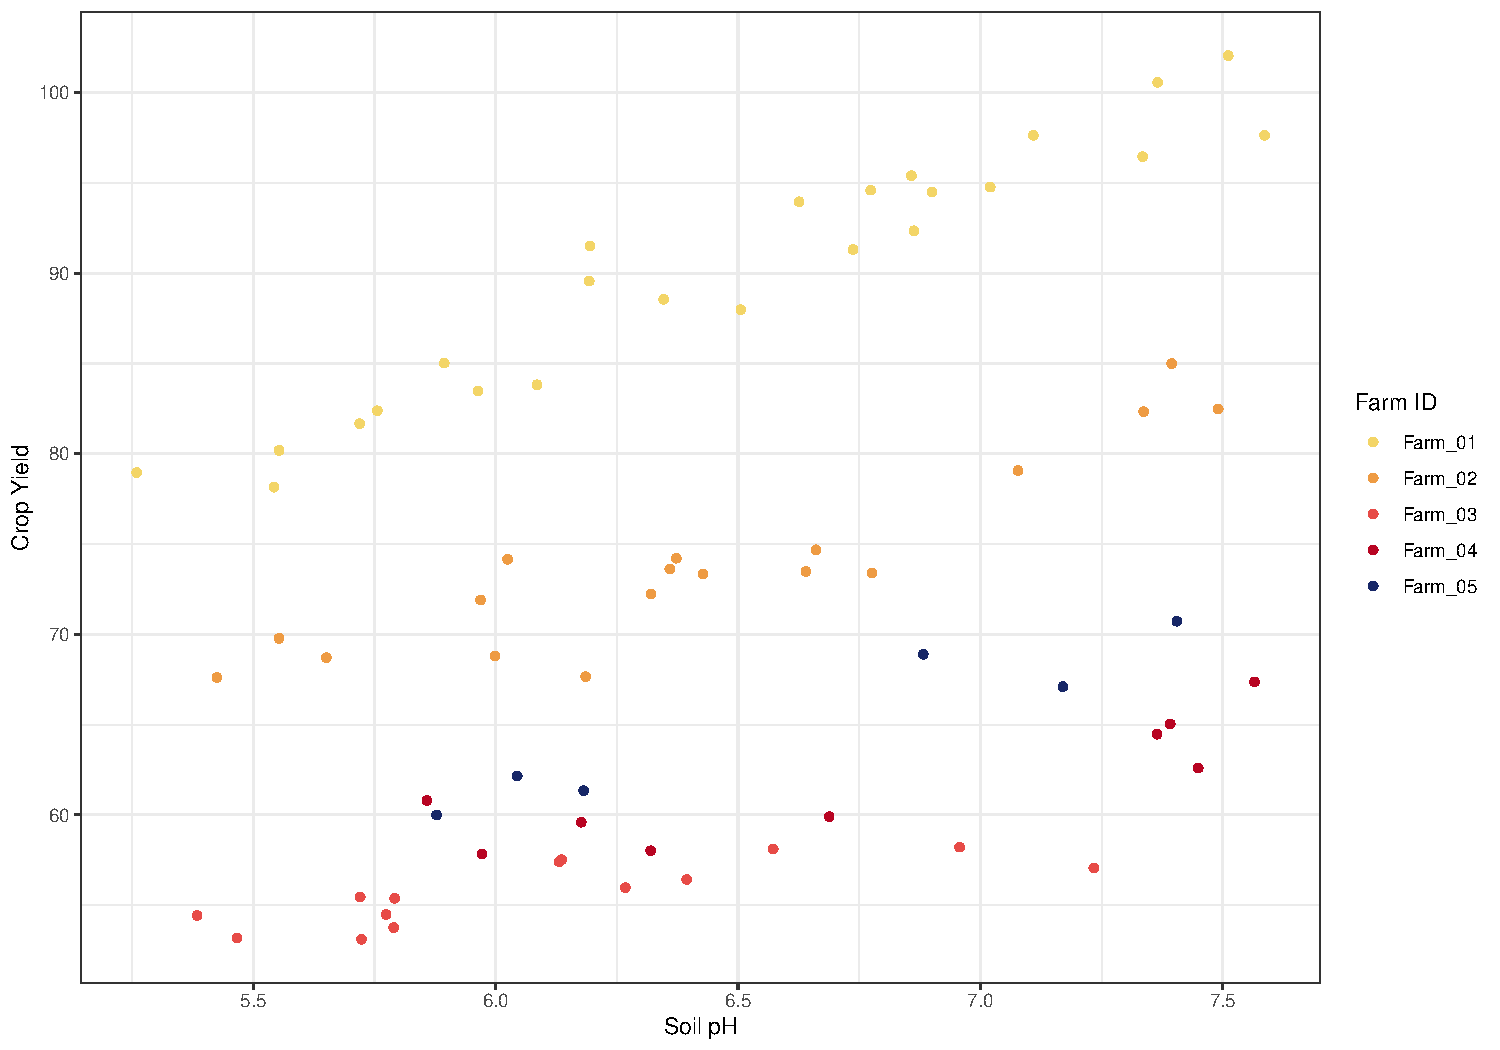
\includegraphics{mixed-effects-workshop_files/figure-beamer/fig-soil-data-1.pdf}

}

\caption{\label{fig-soil-data}Simulated data for this example. Each farm
is a different colour}

\end{figure}%
\end{frame}

\begin{frame}{Some intuition on random effects}
\phantomsection\label{some-intuition-on-random-effects}
** APPLET READOUTS **
\end{frame}

\begin{frame}{Formalism!}
\phantomsection\label{formalism}
Let's start with a nice simple model for our data\footnote<.->{\(Y_{ij}\)
  - crop yield in plots \(i\) nested within farm \(j\). \(x_{ij}\) -
  soil pH across same.}:

\begin{equation}
Y_{ij} = \beta_0 + \beta_1 x_{ij} + \epsilon_{ij}
\end{equation}

\pause

We can now think about adding in a random
effect\footnote<.->{$\alpha_j$ is the random effect across $j = 1,\ldots,k$ farms.}
by the following:

\begin{equation}
Y_{ij} = \beta_0 + \beta_1 x_{ij} + \alpha_j + \epsilon_{ij}
\end{equation}

\pause

where\footnote<.->{$\epsilon_{ij}$ is our random error}

\begin{equation}
\epsilon_{ij} \mathop\sim^{i.i.d.} N(0, \sigma^{2})\text{;    } \alpha_j \mathop\sim^{i.i.d.} N(0, \sigma^{2}_{\alpha})
\end{equation}
\end{frame}

\begin{frame}{Imagine all we knew was that our yields were taken from
different farms}
\phantomsection\label{imagine-all-we-knew-was-that-our-yields-were-taken-from-different-farms}
\begin{figure}[H]

{\centering 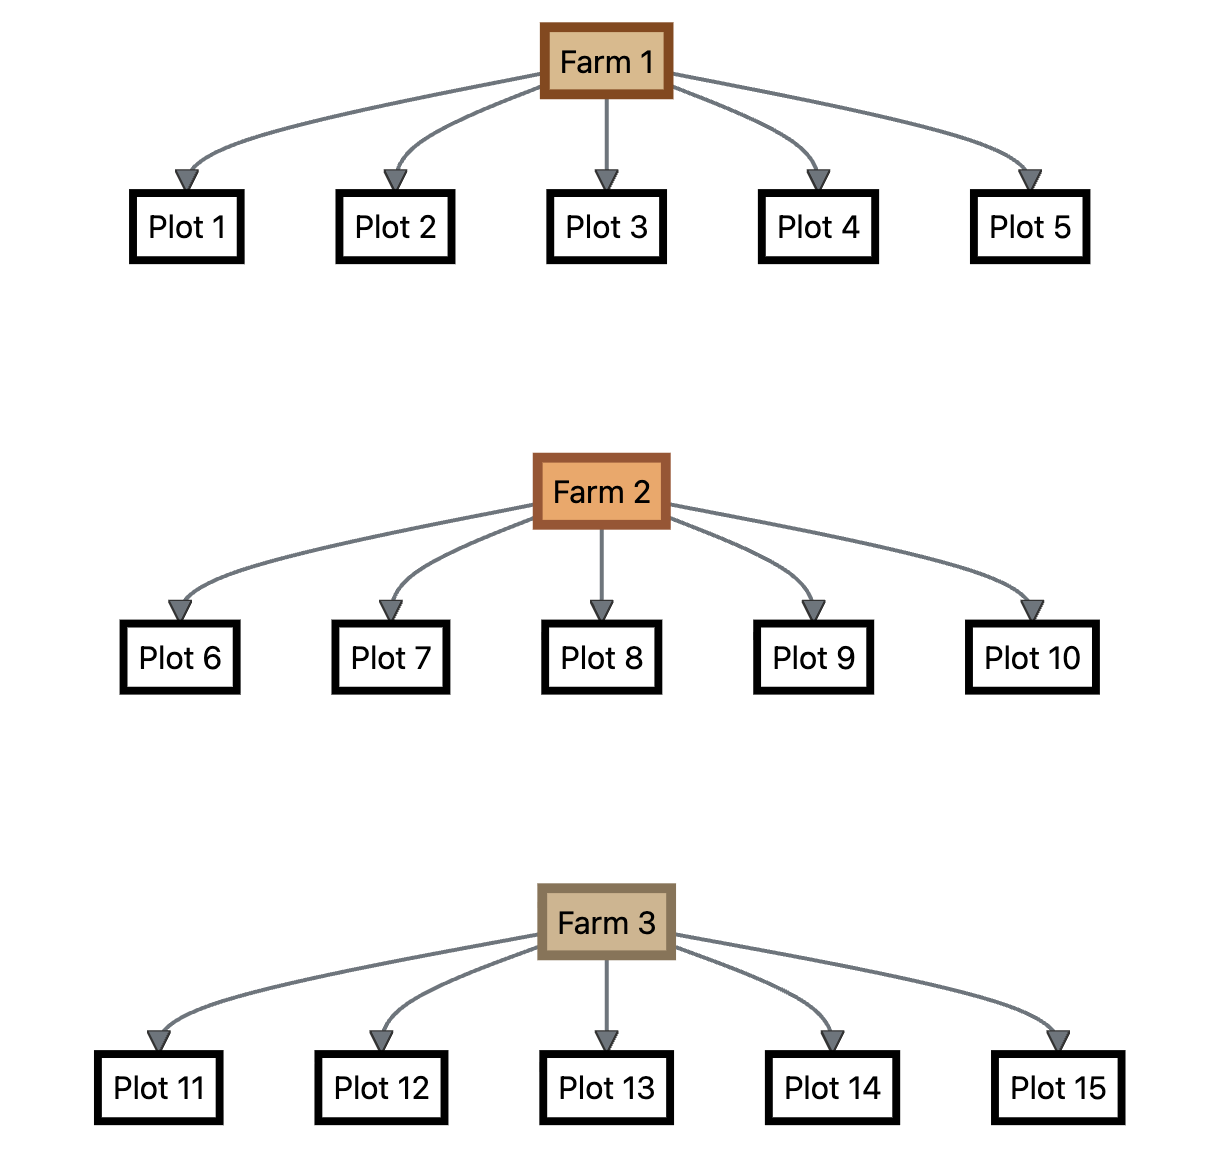
\includegraphics{../assets/images/farms.png}

}

\caption{Visual intuition for how our data are clustered}

\end{figure}%

\textbf{How could we figure out how much variance was clustered within
farms?}
\end{frame}

\begin{frame}{We can start with just our random effect}
\phantomsection\label{we-can-start-with-just-our-random-effect}
Say we didn't know anything about our predictor variables, so our model
was:

\begin{equation}
Y_{ij} = \beta_0 + \alpha_j + \epsilon_{ij}
\end{equation}

\pause

This means that with our simple model, we have the expected value being

\begin{equation}
\begin{aligned}
E[\alpha_{j}] &= \uncover<3->{0} \\
E[Y_{ij}] &= \uncover<3->{\beta_0}
\end{aligned}
\end{equation}

\pause

\uncover<4->{
And the variance is then in turn 

\begin{equation}
\text{Var}(Y_{ij}) = \sigma_{\alpha}^2 + \sigma^2.
\end{equation}
}
\end{frame}

\begin{frame}{Correlation structure}
\phantomsection\label{correlation-structure}
And we get left with this very convenient correlation structure:

\begin{equation}
\text{Cor}(Y_{ij},Y_{i'j'}) =
\begin{cases}
0 & j \neq j' \\
\sigma^2_{\alpha}/(\sigma^2_{\alpha} + \sigma^2) & j = j',\, i \neq i' \\
1 & j = j',\, i = i'
\end{cases}
\end{equation}
\end{frame}

\begin{frame}{Correlation structure}
\phantomsection\label{correlation-structure-1}
Or, if we return to our model including the fixed effect
\footnote<.->{This is the same structure, but $\sigma^2_\alpha$, $\sigma^2$ are now variances after accounting for $x$, and so won't take the same values as they would have on the previous slide.}
\[Y_{ij} = \beta_0 + \beta_1 x_{ij} + \alpha_j + \epsilon_{ij}\]

\begin{equation}
\text{Cor}(Y_{ij},Y_{i'j'} \mid \mathbf{X}) =
\begin{cases}
0 & j \neq j' \\
\sigma^2_{\alpha}/(\sigma^2_{\alpha} + \sigma^2) & j = j',\, i \neq i' \\
1 & j = j',\, i = i'
\end{cases}
\end{equation}

\pause

\begin{center}
\textbf{But why does this matter??}
\end{center}

\pause

\begin{center}
\textbf{\textcolor{red}{Because this is central to understanding the inference on this outcome of interest!}}
\end{center}
\end{frame}

\begin{frame}{This correlation quantity is known as the ICC (intraclass
correlation)}
\phantomsection\label{this-correlation-quantity-is-known-as-the-icc-intraclass-correlation}
\begin{equation}
ICC = \sigma^2_{\alpha}/(\sigma^2_{\alpha} + \sigma^2)
\end{equation}

\vspace{10mm}

\begin{center}
This expression quantifies how much variation comes from \textit{between} farms. If the ICC is large, observations from the \textit{same} farm are much more similar than observations from \textit{different} farms.
\end{center}
\end{frame}

\begin{frame}[fragile]{Let's fit a mixed-effects model!}
\phantomsection\label{lets-fit-a-mixed-effects-model}
\begin{equation}
Y_{ij} = \beta_0 + \beta_1 x_{ij} + \alpha_j + \epsilon_{ij}
\end{equation}

\begin{Shaded}
\begin{Highlighting}[]
\NormalTok{mod }\OtherTok{\textless{}{-}}\NormalTok{ lme4}\SpecialCharTok{::}\FunctionTok{lmer}\NormalTok{(crop\_yield }\SpecialCharTok{\textasciitilde{}}\NormalTok{ soil\_pH }\SpecialCharTok{+}\NormalTok{ (}\DecValTok{1}\SpecialCharTok{|}\NormalTok{farm\_id), }\AttributeTok{data =}\NormalTok{ crop)}
\end{Highlighting}
\end{Shaded}
\end{frame}

\begin{frame}[fragile]{Let's fit a mixed-effects model!}
\phantomsection\label{lets-fit-a-mixed-effects-model-1}
\begin{columns}[T]
\begin{column}{0.48\textwidth}
\begin{verbatim}
Linear mixed model fit by REML ['lmerMod']
Formula: crop_yield ~ soil_pH + (1 | farm_id)
   Data: crop

REML criterion at convergence: 970.2

Random effects:
 Groups   Name        Variance Std.Dev.
 farm_id  (Intercept) 180.988  13.453  
 Residual               7.271   2.697  
Number of obs: 185, groups:  farm_id, 15

Fixed effects:
            Estimate Std. Error t value
(Intercept)  26.9142     3.9787   6.765
soil_pH       6.0386     0.2984  20.235
\end{verbatim}
\end{column}

\begin{column}{0.3\textwidth}
\vspace{3.5em}

What's going on here? We have:

\begin{enumerate}
\tightlist
\item
  Our model formula
\item
  Intercept level variance
\item
  Residual variance
\item
  Our point estimate (and variance) of our soil pH
\end{enumerate}
\end{column}
\end{columns}
\end{frame}

\begin{frame}[fragile]{How should we read this output?}
\phantomsection\label{how-should-we-read-this-output}
We can map those back to our equation that we're fitting!

\vspace{0.5em}

\begin{longtable}[]{@{}lll@{}}
\toprule\noalign{}
\texttt{lme4} output & Math & Estimate Value \\
\midrule\noalign{}
\endhead
\texttt{farm\_id\ (Intercept)} Variance & \(\sigma^2_\alpha\) &
180.99 \\
\texttt{Residual} Variance & \(\sigma^2\) & 7.27 \\
\texttt{(Intercept)} Estimate & \(\beta_0\) & 26.91 \\
\texttt{soil\_pH} Estimate & \(\beta_1\) & 6.04 \\
\bottomrule\noalign{}
\end{longtable}

\pause

It's important to note here that we are not actually \emph{estimating}
the intercepts per farm, we're only estimating the two variance
parameters.

\pause

\begin{center}
\textbf{\textcolor{red}{But then, where do we get the intercepts from??}}
\end{center}
\end{frame}

\begin{frame}[fragile]{So where are the farm intercepts?}
\phantomsection\label{so-where-are-the-farm-intercepts}
\emph{{[}TODO: not estimated as parameters; \emph{predicted} afterwards
from the estimated \(\hat\sigma^2_\alpha\), \(\hat\sigma^2\),
\(\hat\beta\)s{]}}

\[\hat\alpha_j = \lambda_j \left(\bar y_j - \hat\beta_0 - \hat\beta_1 \bar x_j\right), \qquad
\lambda_j = \frac{\hat\sigma^2_\alpha}{\hat\sigma^2_\alpha + \hat\sigma^2 / n_j}\]

\pause

\small

\begin{Shaded}
\begin{Highlighting}[]
\FunctionTok{head}\NormalTok{(}\FunctionTok{ranef}\NormalTok{(mod)}\SpecialCharTok{$}\NormalTok{farm\_id, }\DecValTok{3}\NormalTok{)   }\CommentTok{\# farm deviations, alpha\_j}
\end{Highlighting}
\end{Shaded}

\begin{verbatim}
        (Intercept)
Farm_01   24.856129
Farm_02    8.682289
Farm_03  -17.843012
\end{verbatim}

\begin{Shaded}
\begin{Highlighting}[]
\FunctionTok{head}\NormalTok{(}\FunctionTok{coef}\NormalTok{(mod)}\SpecialCharTok{$}\NormalTok{farm\_id, }\DecValTok{3}\NormalTok{)    }\CommentTok{\# beta\_0 + alpha\_j, and beta\_1}
\end{Highlighting}
\end{Shaded}

\begin{verbatim}
        (Intercept)  soil_pH
Farm_01   51.770290 6.038642
Farm_02   35.596449 6.038642
Farm_03    9.071148 6.038642
\end{verbatim}

\normalsize

\emph{{[}TODO: \(\lambda_j\) is between 0 and 1: farms with few plots or
noisy data get pulled toward the average. We'll see this ``shrinkage''
later{]}}
\end{frame}



\end{document}
